\section{Code Design}
\label{Sect:CodeDesign}

\subsection{General Code Structure}

The main body of the tracker code is implemented as three distinct MAUS map modules and, at present, one reducer module.  There also exist various helpful top-level user tools, and the tracker geometry, calibration and configuration files. A diagram showing the tracker software data flow with the corresponding modules is shown in figure~\ref{Fig:DataFlow}, with the following sections expanding on each area.

\begin{figure}[htb]
    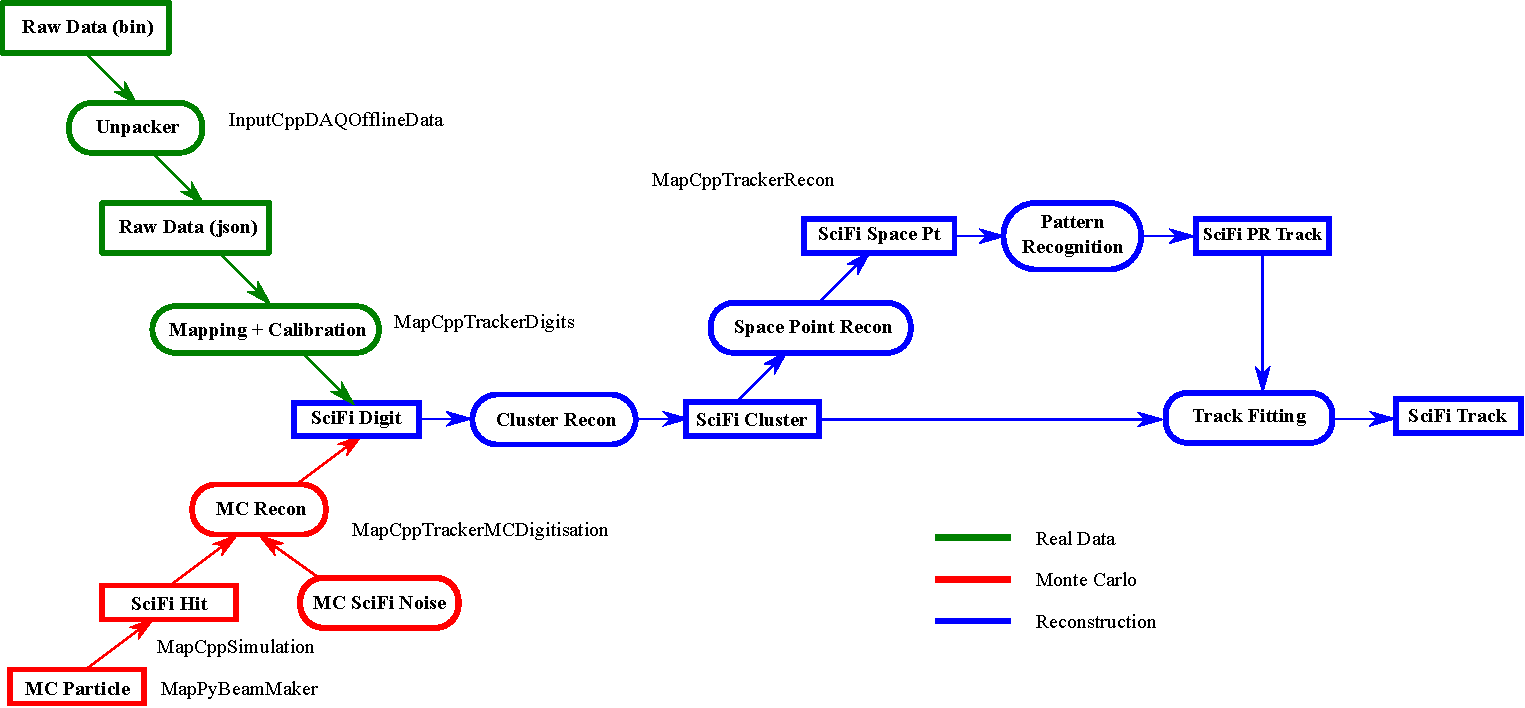
\includegraphics[width=1.0\textwidth]{detectors/tracker/06-CodeDesign/Figures/DataFlow.pdf}
    \caption{Schematic of the tracker software data showing MC and Real data input, and subsequent reconstruction. MAUS modules corresponding to given process are indicated (MapCppTrackerRecon encompasses all of the reconstruction, shown in blue).  Once digits have been formed, reconstruction is agnostic as to whether the MC or Real path was followed.}
    \label{Fig:DataFlow}
\end{figure}

\subsubsection{MapCppTrackerDigits}
This map is used to digitise real data.  It calls on additional functionality from the RealDataDigitisation class, which is stored in \verb;src/common_cpp/Recon/SciFi;.

\subsubsection{MapCppTrackerMCDigitisation}
This map is used to digitise Monte Carlo data.

\subsubsection{MapCppTrackerRecon}
This map performs the main reconstruction work, moving from digits to cluster to spacepoints to pattern recognition tracks, and finally full Kalman tracks. Most work is farmed out to backend C++ classes. The following are the top level classes for each stage of the reconstruction, and are stored in \verb;src/common_cpp/Recon/SciFi;:

\begin{itemize}
 \item SciFiClusterRecon - cluster reconstruction from digits
 \item SciFiSpacepointRecon - spacepoint reconstruction from cluster
 \item PatternRecognition - association of spacepoints to tracks, and crude initial track fit
\end{itemize}

The backend classes for the final track fit are stored under \verb;src/common_cpp/Recon/Kalman; and  \verb;src/common_cpp/Recon/Bayes;, the top level class being KalmanTrackFit.  Other classes used include:

\begin{itemize}
 \item KalmanFilter
 \item KalmanHelicalPropagator
 \item KalmanStraightPropagator
 \item KalmanState
 \item KalmanSeed
\end{itemize}



